\documentclass{article}

\usepackage{graphicx}
\usepackage{tikz}
\usepackage{tikzsymbols}
\usetikzlibrary{calc,patterns,shapes.geometric}
\pagestyle{empty}
\usepackage[margin=0pt]{geometry}
\geometry{papersize={14in,12in}}

\def\centerarc[#1](#2)(#3:#4:#5){\draw[#1] ($(#2)+({#5*cos(#3)},{#5*sin(#3)})$) arc (#3:#4:#5);}

\begin{document}
	\begin{figure}
		\centering
		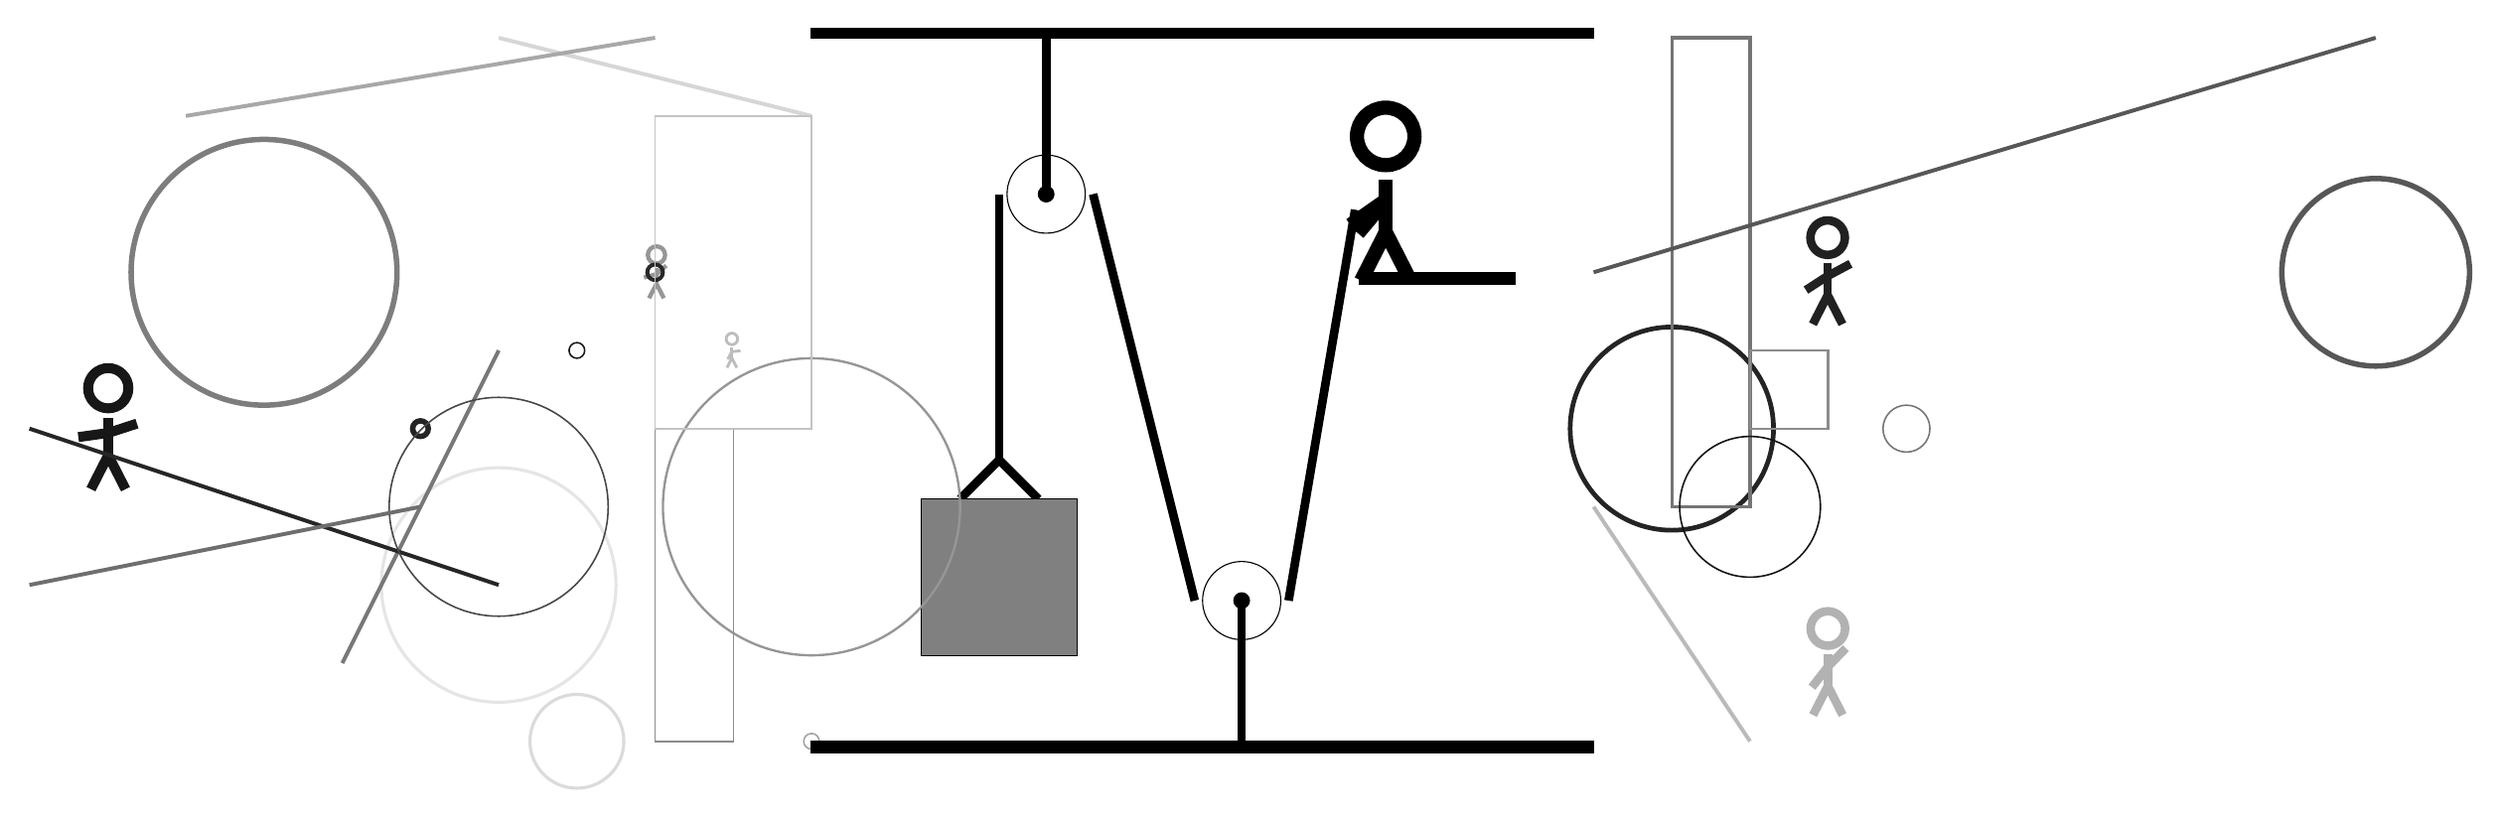
\begin{tikzpicture}
			%%%%% START %%%%%
			
			\draw[fill=black] (-2, 9) rectangle (8, 9.125);
			
			\draw (3.5, 1.8) circle (0.5);
			\draw[fill=black] (3.5, 1.8) circle (0.1);
			\draw[line width=1.1mm] (3.5, 1.8) -- (3.5, 0);
			
			\draw (1, 7) circle (0.5);
			\draw[fill=black] (1, 7) circle (0.1);
			\draw[line width=1.1mm] (1, 9) -- (1, 7);
			
			\draw[line width=1.1mm](-0.1, 3.1) --  (0.4, 3.6) -- (0.9, 3.1);
			\draw[fill=black!50] (-0.6, 3.1) rectangle (1.4, 1.1);
			
			\draw [line width=0.4mm, color=black!10](-6, 2) circle (1.5);
			
			\draw[line width=0.7mm, color=black!50] (-4, 9) rectangle (-4, 9);
			\draw [line width=0.2mm, color=black!36](-2, 0) circle (0.1);
			\draw [line width=0.4mm, color=black!14](-5, 0) circle (0.6);
			\draw[line width=0.5mm, color=black!53](-6, 5) -- (-8, 1);
			\draw[line width=0.5mm, color=black!27](8, 3) -- (10, 0);
			\node[line width=0.6mm, color=black!41] at (-4, 6) {\Strichmaxerl[3][15][41]};
			\draw [line width=0.2mm, color=black!54](12, 4) circle (0.3);
			\draw [line width=0.6mm, color=black!86](9, 4) circle (1.3);
			
			\draw [line width=0.3mm, color=black!41](-2, 3) circle (1.9);
			\draw[line width=0.2mm, color=black!19] (-4, 5) rectangle (-4, 3);
			\node[line width=0.3mm, color=black!26] at (-3, 5) {\Strichmaxerl[2][61][6]};
			\draw[line width=0.4mm, color=black!54] (10, 9) rectangle (9, 3);
			
			\draw [line width=0.7mm, color=black!86](-7, 4) circle (0.1);
			\draw [line width=0.2mm, color=black!91](-5, 5) circle (0.1);
			\node[line width=0.4mm, color=black!87] at (11, 6) {\Strichmaxerl[6][33][28]};
			
			\draw[line width=0.2mm, color=black!45] (-4, 0) rectangle (-3, 4);
			\draw [line width=0.2mm, color=black!93](10, 3) circle (0.9);
			\draw[line width=0.5mm, color=black!16](-2, 8) -- (-6, 9);
			\draw[line width=0.5mm, color=black!66](8, 6) -- (18, 9);
			\draw [line width=0.5mm, color=black!84](-4, 6) circle (0.1);
			
			\draw[line width=0.3mm, color=black!45] (10, 4) rectangle (11, 5);
			\node[line width=0.3mm, color=black!30] at (11, 1) {\Strichmaxerl[6][52][46]};
			\node[line width=0.3mm, color=black!91] at (-11, 4) {\Strichmaxerl[7][8][18]};
			\draw [line width=0.7mm, color=black!51](-9, 6) circle (1.7);
			
			\draw [line width=0.7mm, color=black!66](18, 6) circle (1.2);
			\draw[line width=0.5mm, color=black!85](-6, 2) -- (-12, 4);
			\draw [line width=0.2mm, color=black!72](-6, 3) circle (1.4);
			\draw[line width=0.5mm, color=black!34](-4, 9) -- (-10, 8);
			\draw[line width=0.2mm, color=black!23] (-2, 8) rectangle (-4, 4);
			\draw[line width=0.5mm, color=black!57](-7, 3) -- (-12, 2);
			
			
			\draw[line width=1.1mm](0.4, 7) -- (0.4, 3.6);
			\centerarc[line width=1.1mm](1, 7)(180:0:0.6)
			\draw[line width=1.1mm](1.6, 7) -- (2.9, 1.8);
			\centerarc[line width=1.1mm](3.5, 1.8)(180:360:0.6)
			\draw[line width=1.1mm](4.1, 1.8) -- (4.95, 6.8);
			
			\node at (5.3, 7) {\Strichmaxerl[10][35][-130]};
			\draw[fill=black] (5, 6) rectangle (7, 5.85);
			
			\draw[fill=black] (-2, 0) rectangle (8, -0.15);
			
			%%%%% END %%%%%
		\end{tikzpicture}
	\end{figure}	
\end{document}